In the following section we present the complete \emph{Class Diagram} in \autoref{ClassDiagram1} and the Alloy code written using the \emph{Alloy Analyzer 4.2} tool given by MIT.\\
At the end there is also an image of an instance found in \autoref{AlloyInstance}.

\begin{figure}[H]
\begin{center}
		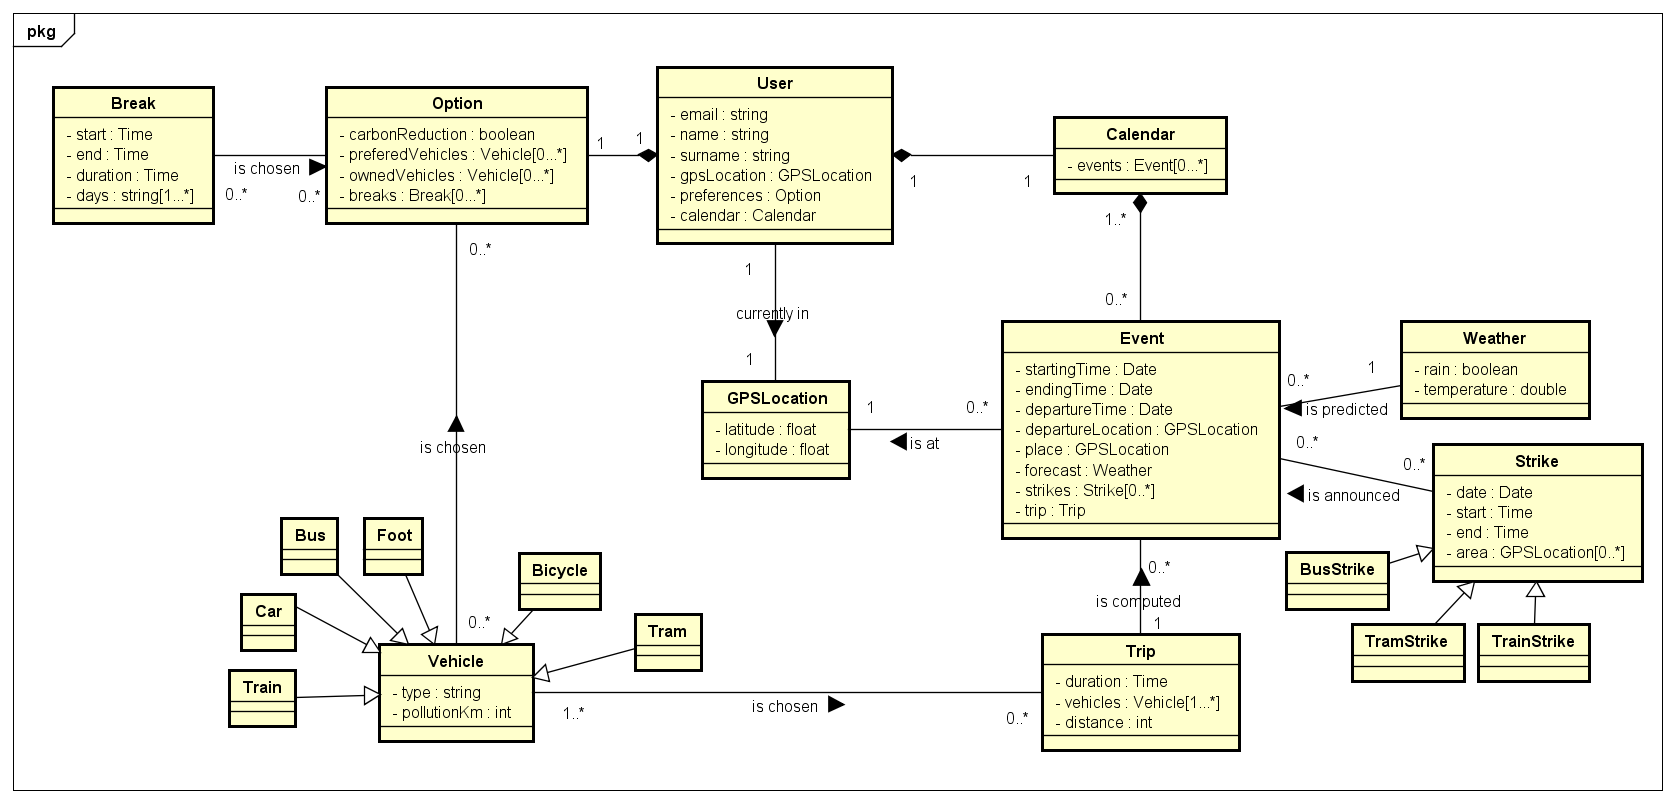
\includegraphics[width=\textwidth, angle=90,keepaspectratio=true]{Img/ClassDiagram1}
		\caption{Class diagram illustrating the structure of the system-to-be.}
		\label{ClassDiagram1}
\end{center}
\end{figure}

\newpage
\lstset{
    language=alloy,
    numbers=left,
    numberstyle=\tiny,
    stepnumber=2,
    tabsize=4,
    keywordstyle=\color{alloy-keyword}\bfseries,
    commentstyle=\color{alloy-comment},
    stringstyle=\color{alloy-string},
    basicstyle=\small\fontfamily{pcr}\selectfont,
}

\lstinputlisting{Files/TravlendarAlloy.als}
\vfill
\subsection{Alloy Execution Result}
The following is the result of the execution of the checks:\\
\begin{figure}[H]
\begin{center}
		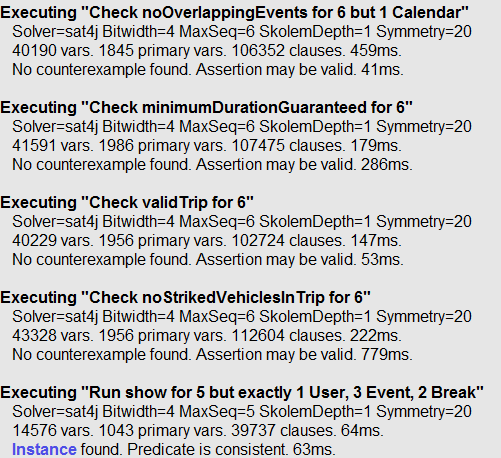
\includegraphics[width=\textwidth, keepaspectratio=true]{Img/AlloyEx}
		\caption{Alloy's Execution Result}
\end{center}
\end{figure}
\clearpage
\subsection*{Instance Found}

\begin{figure}[H]
\begin{center}
	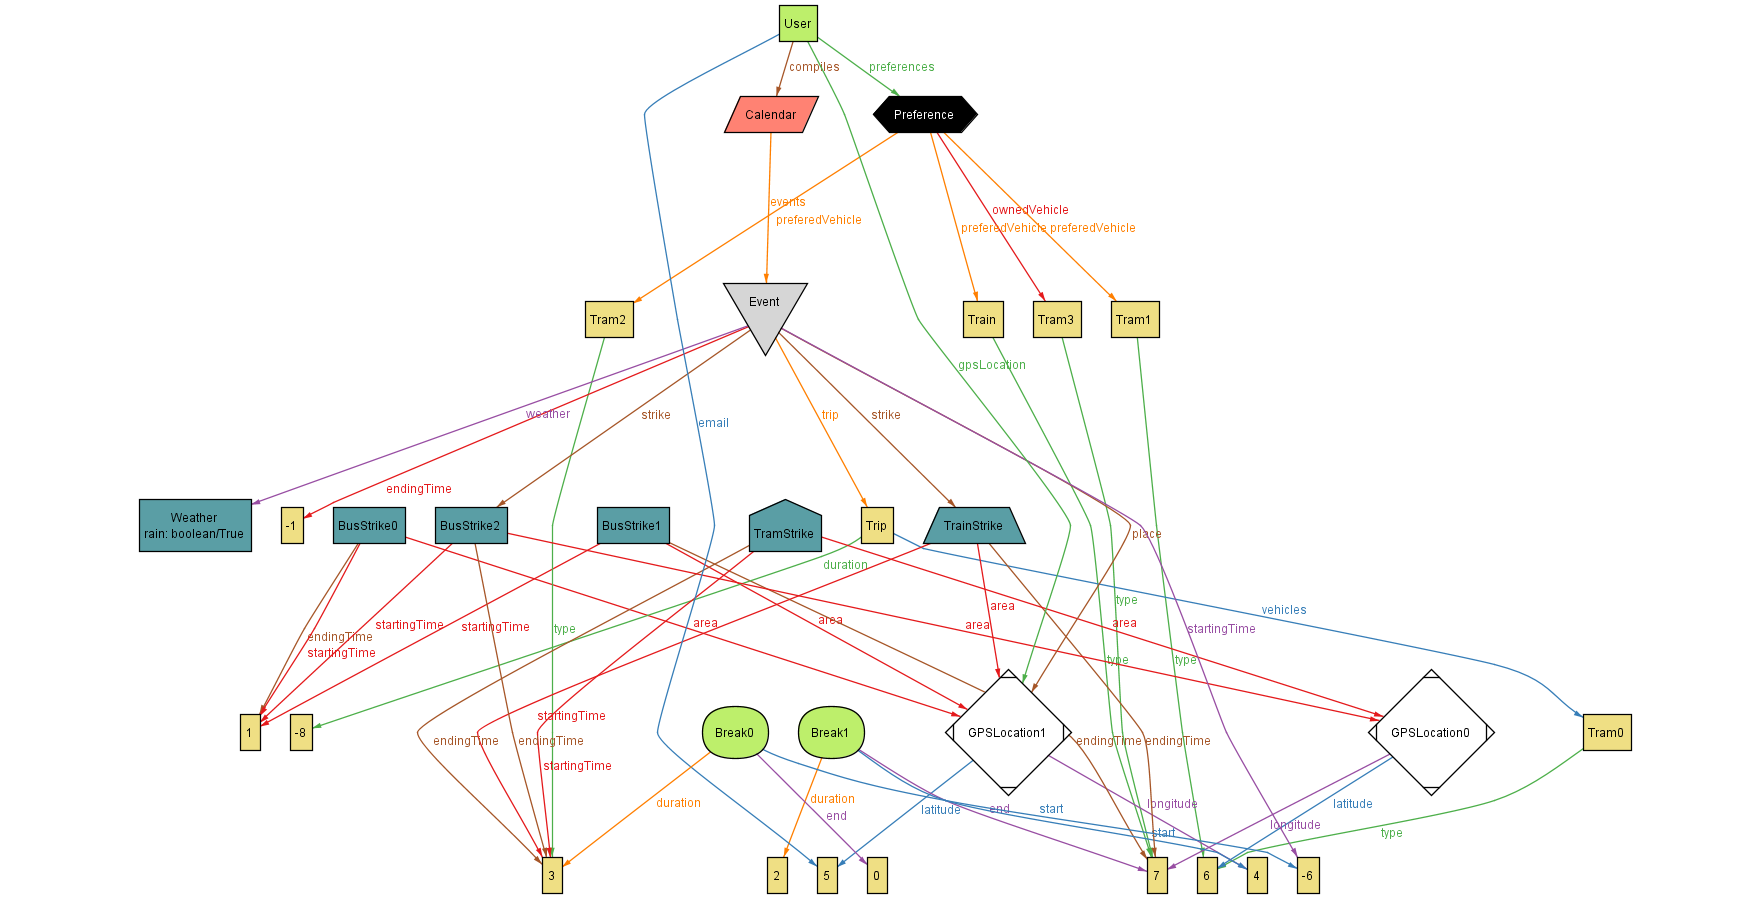
\includegraphics[width=\textwidth, height=\textheight, angle=90, keepaspectratio=true]{Img/AlloyInstance}
	\caption{Instance of Alloy found.}
	\label{AlloyInstance}
\end{center}
\end{figure}

